\documentclass{beamer}
%\usetheme{Ilmenau}
%\usecolortheme{beaver}

\usepackage[slovak,american]{babel}
\usepackage[utf8]{inputenc}
\usepackage{graphicx}
\usepackage{adjustbox}
\usepackage{xcolor}
\usepackage{mathrsfs}
 
 \newsavebox\MBox
\newcommand\Cline[2][red]{{\sbox\MBox{$#2$}%
  \rlap{\usebox\MBox}\color{#1}\rule[-2.2\dp\MBox]{\wd\MBox}{1pt}}}

%\usefonttheme{serif}

%\definecolor{UKOrange}{HTML}{ef9424} %
\definecolor{UKOrange}{HTML}{7a2c18} %
\definecolor{UKBrown}{HTML}{a96d5e} %
\definecolor{UKLight}{HTML}{d8b6ab} %
\definecolor{UKDark}{HTML}{7a4f44}
\definecolor{UKDarker}{HTML}{4d312b} 
\definecolor{UKDarkest}{HTML}{2e1e1a}
\definecolor{UKRed}{HTML}{bf1f1c}

\setbeamertemplate{footline}[frame number]{}
\setbeamertemplate{navigation symbols}{}

%\usecolortheme{beaver}
\setbeamertemplate{itemize item}[square]
\setbeamercolor{itemize item}{fg = UKBrown}
\setbeamercolor{itemize subitem}{fg = UKLight}
\setbeamercolor{enumerate item}{fg = UKDark}

\setbeamercolor{footnote}{fg=UKLight}
\setbeamercolor{footnote mark}{fg=UKLight}
\setbeamerfont{footnote}{size=\tiny}
\renewcommand\footnoterule{}

\usetheme{default}
\beamertemplatenavigationsymbolsempty
\setbeamercolor{title}{fg=white, bg=UKBrown}
\setbeamercolor{frametitle}{fg=white, bg=UKBrown}
\setbeamercolor{block title}{bg=UKBrown, fg= white}
\setbeamercolor{block body}{bg =UKLight, fg = UKDarkest}

\setbeamercolor{block title alerted}{bg=UKOrange, fg= white}
\setbeamercolor{block body alerted}{bg =UKLight, fg = UKDarkest}


%\setbeamercolor{section in toc}{fg = UKBrown}
%\setbeamercolor{section in toc}{fg = UKDarkest}

% odstrani gulicky
\renewcommand*{\slideentry}[6]{}

\useoutertheme[subsection=false]{miniframes}
\AtBeginSection[]{\subsection{}}

\setbeamercolor{below lower separation line head}{bg=UKDark}
\addtobeamertemplate{headline}{}{%
  \begin{beamercolorbox}[colsep=0.5pt]{below lower separation line head}
  \end{beamercolorbox}
}
%\setbeamercolor*{mini frame}{fg=white,bg=UKRosy}
\setbeamercolor{section in head/foot}{fg=UKLight, bg=UKDark}

\usepackage{etoolbox}
\makeatletter
\preto{\@verbatim}{\topsep=0pt \partopsep=0pt }
\makeatother

%\setbeamertemplate{itemize/enumerate body begin}{\normalsize}
%\setbeamertemplate{itemize/enumerate subbody begin}{\normalsize}




%\newcommand{\codeblock}[2]{ \begin{block}{#1} \begin{verbatim}#2\end{verbatim}\end{block}}

%\defbeamertemplate*{title page}{customized}[1][]
%{
%  \begin{centering}
%    \begin{beamercolorbox}[sep=8pt,center]{title}
%      \usebeamerfont{title}\inserttitle
%    \end{beamercolorbox}
%  \end{centering}
%  \bigskip
%
%\begin{columns}[onlytextwidth,T]
%
%
%  \column{27mm}
%  \includegraphics[width=27mm]{images/logoFMFI.png}
%  
%  \column{\dimexpr\linewidth-54mm-6mm}
%  \centering
%  \vspace{5mm}  
%  \usebeamerfont{author}\insertauthor\par
%  \vspace{5mm}
%  \usebeamerfont{institute}\insertinstitute\par
%
%  \column{27mm}
%  \includegraphics[width=27mm]{images/logoUK.png}  
%\end{columns}
%\centering
%\vspace{7mm}
%  \usebeamerfont{date}\insertdate\par
%}

\DeclareMathOperator*{\argmin}{arg\,min}
\newcommand{\e}[1]{$\cdot 10^{#1}$}

%\newcommand{\codeblock}[2]{ \begin{block}{#1} \begin{verbatim}#2\end{verbatim}\end{block}}



\title[10. cvičenie]{Pokročilé spracovanie obrazu - Segmentácia}
\author[Kocur]{Ing. Viktor Kocur \\{\small viktor.kocur@fmph.uniba.sk}}
\institute{DAI FMFI UK}
\date{27.11.2017}

\begin{document}
\selectlanguage{slovak}


\begin{frame}

  \titlepage

\end{frame}

\section{Segmentácia}
\subsection{O čo ide}

\begin{frame}
\frametitle{Cieľ segmentácie}
\begin{block}{Cieľ segmentácie}
Cieľom segmentácie je rozdeliť obrázok na disjunktné oblasti, tak že jednotlivé oblasti zodpovedajú samostatným objektom/útvarom.
\end{block}

\begin{block}{Čiastočná segmentácia}
Nie vždy je možné rozdeliť obraz na jednotlivé objekty/útvary. Niekedy nám však stačí čiastočná segmentácia. V takom prípade môže byť segmentovaný, len nejaký objekt, alebo skupina objektov.
\end{block}
\end{frame}

\begin{frame}
\frametitle{Pôvodný obrázok}
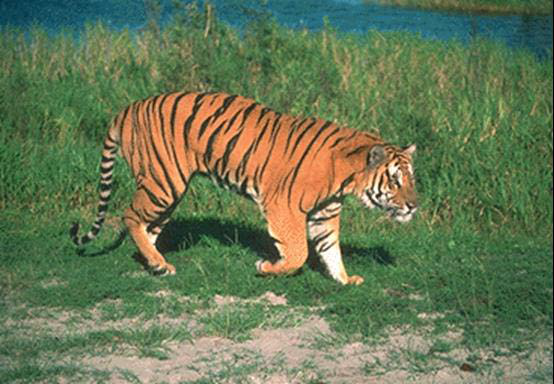
\includegraphics[width=\textwidth]{tiger.png}
\end{frame}

\begin{frame}
\frametitle{Segmentovaný}
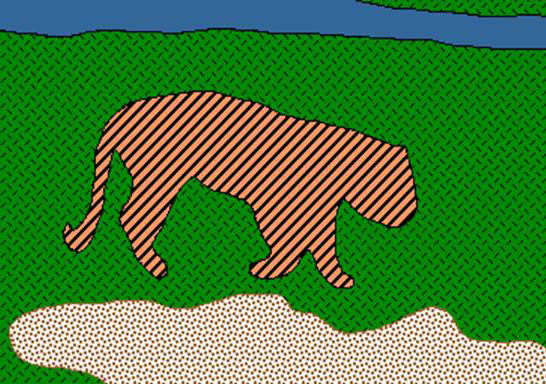
\includegraphics[width=\textwidth]{tiger_segmented.png}
\end{frame}



\section{k-means clustering}

\subsection{Algoritmus}

\begin{frame}
\frametitle{k-means clustering}

\begin{block}{k-means}
k-means clustering je metóda, ktorá zo súboru vektorov vytvorí k skupín, ktoré predstavujú jeden zhluk.
\end{block}

\begin{block}{Postup}
\begin{itemize}
\item V požadovanom vektorovom priestore náhodne rozmiestnim k 'centroidov'
\item Každý vektor priradím centroidu ktorému je najbližšie
\item Centroidy posunieme, tak ich nové pozície budú ťažiská ich priradených vektorov
\item Opakujeme 2. a 3. bod kým sa centroidy posúvajú
\end{itemize}
\end{block}
\end{frame}

\begin{frame}
\frametitle{k-means}
\begin{center}
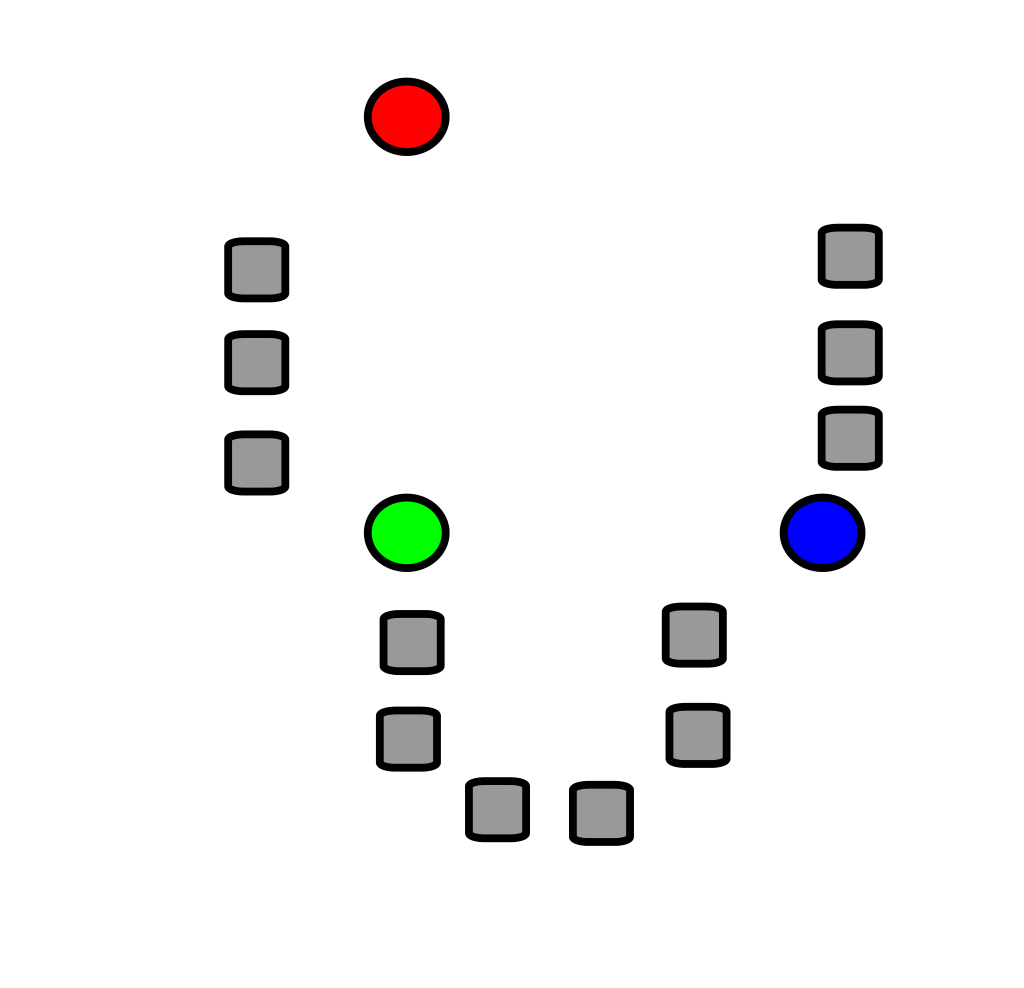
\includegraphics[width=0.8\textwidth]{km1.png}
\end{center}
\end{frame}

\begin{frame}
\frametitle{k-means}
\begin{center}
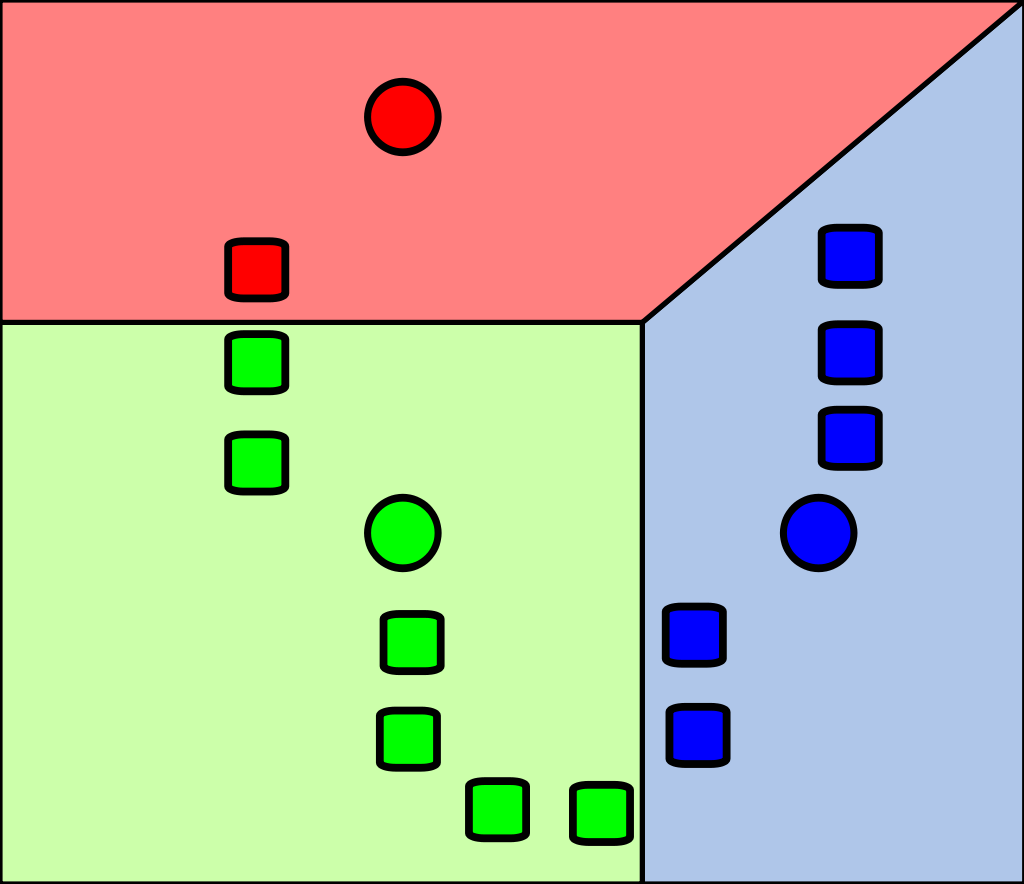
\includegraphics[width=0.8\textwidth]{km2.png}
\end{center}
\end{frame}

\begin{frame}
\frametitle{k-means}
\begin{center}
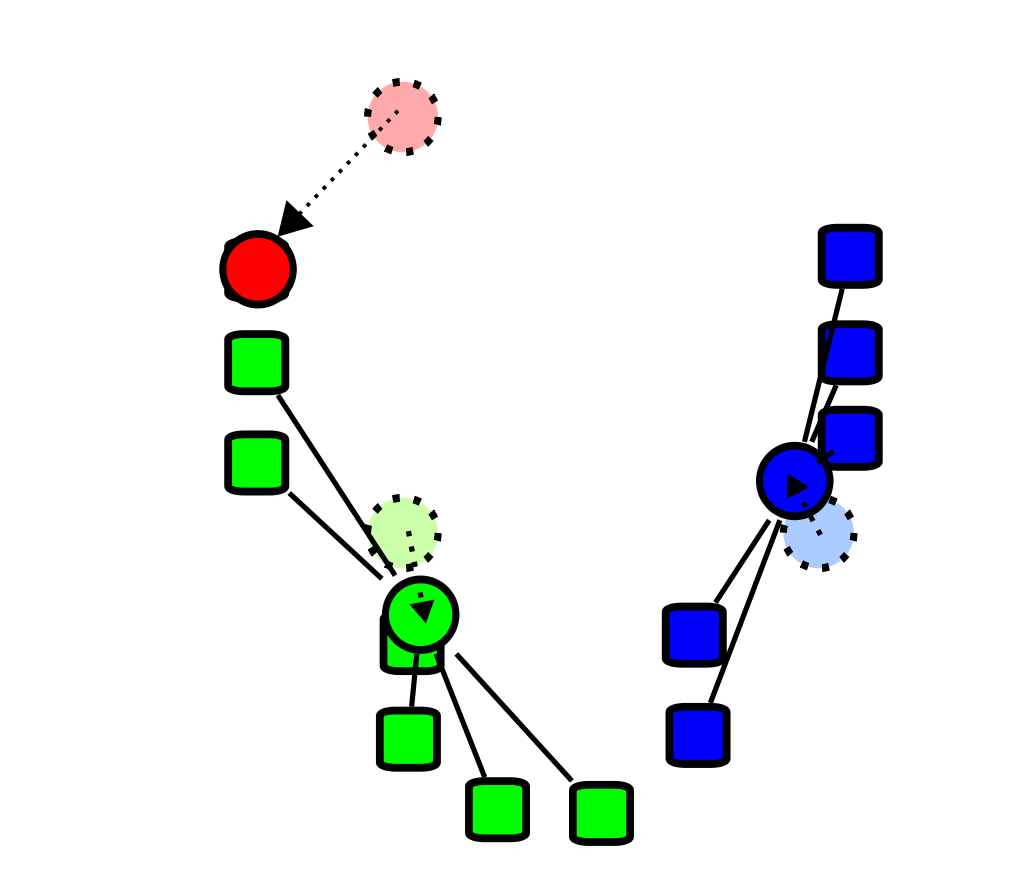
\includegraphics[width=0.8\textwidth]{km3.png}
\end{center}
\end{frame}

\begin{frame}
\frametitle{k-means}
\begin{center}
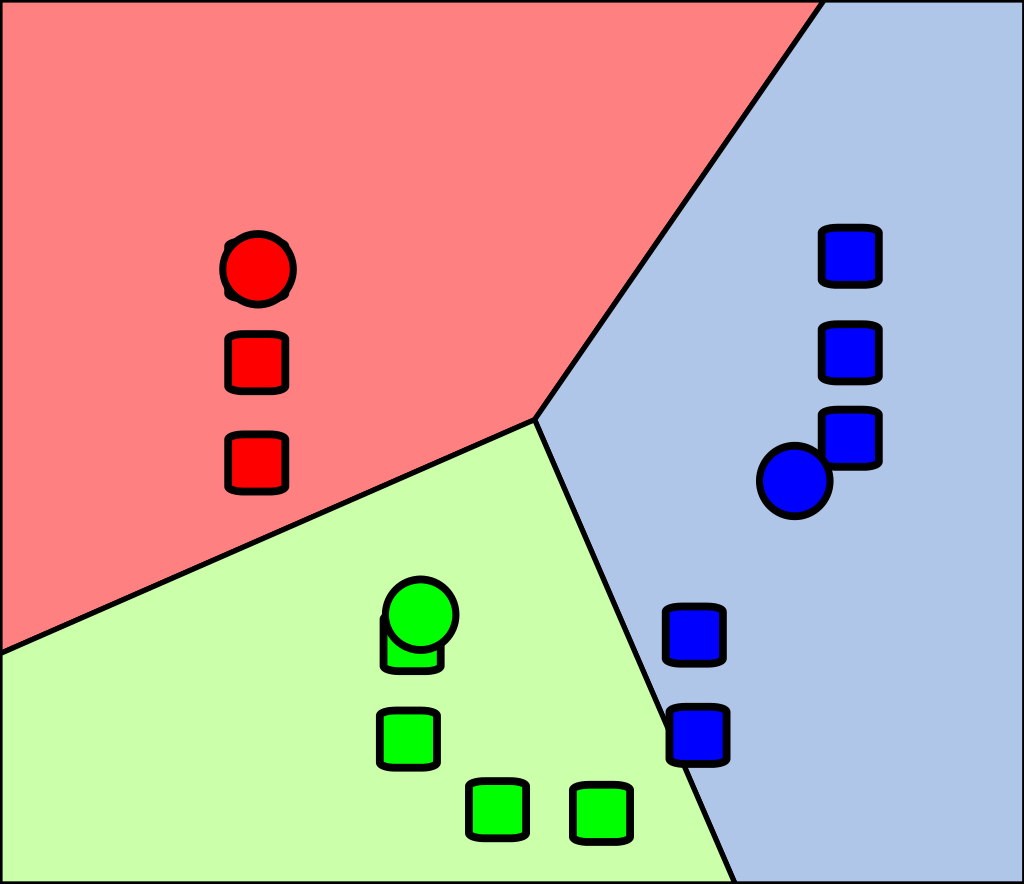
\includegraphics[width=0.8\textwidth]{km4.png}
\end{center}
\end{frame}

\subsection{k-means v Matlabe}

\begin{frame}
\frametitle{k-means v matlabe}
\begin{block}{kmeans}
kmeans(A, k) - pre maticu s n riadkami, z ktorých každý predstavuje jeden vektor vráti vektor dĺžky n ktorého prvky sú hodnoty od 1 po k, podľa toho do ktorého klusteru daný vektor patrí
\end{block}

\begin{block}{Vektory pre segmentáciu obrazu}
Pre obrazy môžeme napríklad segmentovať jednotlivé pixely. Ako ich vektory môžeme zobrať ich pozíciu a farbu.
\end{block}
\end{frame}

\begin{frame}
\frametitle{k-means v matlabe}
\begin{block}{Úloha}
Použite k-means na obrázok zátišia. Ako vektory vezmite farby v Lab priestore.
\end{block}

\begin{block}{Úloha}
Ako vektory použite farbu, ale aj x-ové a y-ové súradnice. Nazabudnite jednotlivé zložky normalizovať.
\end{block}


\begin{block}{meshgrid}
[X, Y] = meshgrid(1:c,1:r) - vytvorí dve matice rozmerov $r \times c$. X obsahuje x-ové súradnice v tejto matici, Y obsahuje y-ové súradnice.
\end{block}
\end{frame}

\section{Graph Cut}
\subsection{Graph Cut}

\begin{frame}
\frametitle{Graph Cut}
\begin{block}{Graph Cut}
Graph Cut je metóda ktorá využíva uživateľský vstup na segmentáciu popredia. Uživateľ označí nejaké pixely ako popredie a pozadie.
\end{block}

\begin{block}{Algoritmus}
Zo všetkých pixelov sa zostrojí graf, každý pixel je spojený so susednými s váhou, ktorá zodpovedá podobnosti pixelov. V grafe sú ešte dva vrcholy jeden reprezentuje popredie a druhý pozadie. Tieto sú prepojené s pixelmi pomocou pravdepodobnosti, že sú z popredia resp. z pozadia. Túto pravdepodobnosť získame pomocou distribúcie farieb v uživateľom ožnačenými pixelmi.  Nakoniec použijeme algoritmus ktorý urobí rez grafom tak, aby minimalizoval energiu, teda váhy hrán ktoré vedú od vrchola popredia k vrcholu pozadia.
\end{block}

\end{frame}

\begin{frame}
\frametitle{Graph Cut}
\begin{block}{Matlab}
Graph Cut sa dá použiť aj v matlabe. V záložke apps si nájdite image segmnenter.
\end{block}
\end{frame}


\section{Jednoduchá segmentácia podľa farby}

\begin{frame}
\frametitle{Jednoduchá segmentácia podľa farby}
\begin{block}{Uživeteľský vstup}
Môžeme použiť vstup od uživateľa aby sme vybrali farbu a následne segmentovali pixely podľa ich vzdialenosti od tejto farby v nejakom farebnom priestore. Ak máme vzdialenosť tak nám stačí určiť vhodný prah a máme segmentovaný obraz.\end{block}

\begin{block}{Priestorová informácia}
Rovnako ako pri k-means môžeme do vzdialenosti zarátať aj priestorovú vzdialenosť.
\end{block}

\begin{block}{Úloha}
Použite tento prístup pre segmentáciu jabĺk, alebo pomarančou v obrázku zátišia. Skúste rôzne farebné priestory. Pridajte informáciu o vzdialenosti pixelov. Využite vyhladzovanie obrazu a morfologicke operácie na zlepšenie výsledku.
\end{block}
\end{frame}

\end{document}

\section{Watershed}

\subsection{Princíp}

\begin{frame}
\frametitle{Princíp}
\begin{block}{Watershed}
Watershed vníma obraz ako topgraifickú mapu a oblasti rozdelí, podľa toho ako by boli rozdelené povodia na mape.
\end{block}

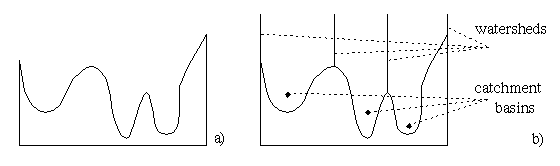
\includegraphics[width=\textwidth]{basins.png}

\begin{block}{Vstup pre watershed}
Watershed je fajn, ale najprv potrebujeme vhodný obraz na získanie povodí.
\end{block}
\end{frame}

\begin{frame}
\frametitle{Princíp}

\begin{block}{imgradient}
imgradient(I) - vráti gradient šedotónového obrázka
\end{block}

\begin{block}{watershed}
watershed(I) - vráti label maticu po aplikácii watershed algoritmu na šedotónový obraz
\end{block}

\begin{block}{label2rgb}
label2rgb(L) - z label matice vytvorí obrázok, kde sú farby určené podľa labelov
\end{block}

\begin{block}{Úloha}
Načítajte si obrázok pears.png, zobrazte si jeho gradient a watershed gradientu
\end{block}

\end{frame}


\subsection{Postup}

\begin{frame}
\frametitle{Postup}
\begin{block}{Postup rozdelíme na časti}
\begin{itemize}
\item Otvorenie a zatvorenie pomocou imreconstruct
\item Nájdenie masky popredia
\item Nájdenie hrebeňov v obraze
\item Vynútenie miním na maske
\item Watershed
\end{itemize}
\end{block}

\begin{block}{Link}
Tento postup je aj na stránke: https://www.mathworks.com/help/images/marker-controlled-watershed-segmentation.html
\end{block}
\end{frame}

\begin{frame}[fragile]
\frametitle{Otvorenie a zatvorenie}
\begin{block}{Kód}
\begin{verbatim}
se = strel('disk',20);
Ioc = imclose(imopen(I,se),se);
Ie = imerode(I,se);
Iobr = imreconstruct(Ie,I);
Iobrd = imdilate(Iobr,se);
Iobrcbr = imreconstruct(imcomplement(Iobrd), ...
    imcomplement(Iobr));
Iobrcbr = imcomplement(Iobrcbr);
\end{verbatim}
\end{block}

\begin{block}{Čo sa udialo}
Realizovali sme operáciu otvorenia a následného zatvorenia, ale za použitia markerov, tj pomocou rekonštrukcie.
\end{block}
\end{frame}

\begin{frame}[fragile]
\frametitle{Otvorenie a zatvorenie}
\begin{block}{Kód}
\begin{verbatim}
fgm = imregionalmax(Iobrcbr);
se2 = strel(ones(5,5));
fgm2 = imclose(fgm,se2);
fgm3 = imerode(fgm2,se2);
fgm4 = bwareaopen(fgm3,20);
\end{verbatim}
\end{block}

\begin{block}{Čo sa udialo}
Vytvorili sme masku popredia z oblastí ktoré sú lokálnymi maximami. Potom sme ju pomocou morfológie upravili a nakoniec sme odstránili oblasti s obsahom menším ako 20 pixelov. 
\end{block}
\end{frame}

\begin{frame}[fragile]
\frametitle{Nájdenie hrebeňov pozadia}
\begin{block}{Kód}
\begin{verbatim}
dist = bwdist(imbinarize(Iobrcbr));
ws1 = watershed(dist);
bgm = ws1 == 0;
\end{verbatim}
\end{block}

\begin{block}{Čo sa udialo}
Zobrali sme širšie popredie a pomocou funkcie bwdistance, sme spočítali pre každý pixel vzdialenosť od najbližšieho pixelu popredia. Na tieto vzdialenosti sme aplikovali watershed a získali sme tak oblasti ktoré sú hrebeňmi.
\end{block}
\end{frame}

\begin{frame}[fragile]
\frametitle{Vynútenie minima a watershed}
\begin{block}{Kód}
\begin{verbatim}
grad = imgradient(I);
grad2 = imimposemin(grad, bgm | fgm4);
L = watershed(grad2);
\end{verbatim}
\end{block}

\begin{block}{Čo sa udialo}
Spojili sme masku miest kde chcme mať 'kotliny' a vynútili sme aby na gradientnom obraze boli lokálne minimá len tam. Týmto spôsobom sa samostatne segmentujú objekty a zároveň aj pozadie bude mať svoje povodie. Nakoniec aplikujeme watershed.
\end{block}
\end{frame}

\begin{frame}[fragile]
\frametitle{Krajšie zobrazenie obrázka}
\begin{block}{Kód}
\begin{verbatim}
figure
imshow(I)
hold on
himage = imshow(Lrgb);
himage.AlphaData = 0.3;
\end{verbatim}
\end{block}

\begin{block}{Čo sa udialo}
Len sme vykreslil obrázok pekným spôsobom.
\end{block}
\end{frame}